\documentclass[tikz,border=10pt]{standalone}
\usepackage{tikz}
\usetikzlibrary{calc}

\begin{document}
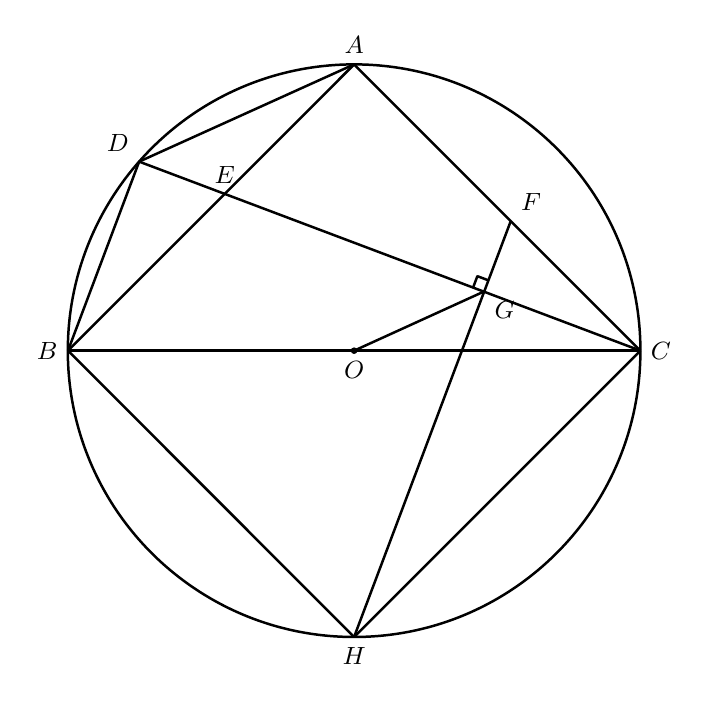
\begin{tikzpicture}[line width=0.9pt, line join=round, scale=1]
  % Coordinates: s = 0.0077 cm/px, origin at circle centre O, y flipped
  \coordinate (O) at (0,0);
  \coordinate (A) at (0,3.636);
  \coordinate (B) at (-3.634,0);
  \coordinate (C) at (3.636,0);
  \coordinate (H) at (0,-3.635);
  \coordinate (D) at (-2.730,2.401);
  \coordinate (E) at (-1.643,1.995);
  \coordinate (G) at (1.653,0.753);
  \coordinate (F) at (1.989,1.645);
  \coordinate (P) at (1.371,0);   % intersection of FH with BC

  % Circle
  \draw (O) circle (3.636);

  % Segments
  \draw (B) -- (C);      % through O
  \draw (A) -- (B);
  \draw (A) -- (C);
  \draw (B) -- (D);
  \draw (D) -- (A);
  \draw (H) -- (B);
  \draw (H) -- (C);
  \draw (D) -- (C);      % through E and G
  \draw (F) -- (H);      % through G and P
  \draw (O) -- (G);

  % Right-angle mark at G (between FH and DC), one mark only
  \coordinate (RP1) at (1.5126,0.806);
  \coordinate (RP2) at (1.7059,0.8933);
  \coordinate (RPc) at (1.5655,0.9463);
  \draw (RP1) -- (RPc) -- (RP2);

  % Centre dot
  \fill (O) circle (1.2pt);

  % Labels (font from style metrics)
  \node[font=\fontsize{9}{10.8}\selectfont, above] at (A) {$A$};
  \node[font=\fontsize{9}{10.8}\selectfont, left] at (B) {$B$};
  \node[font=\fontsize{9}{10.8}\selectfont, right] at (C) {$C$};
  \node[font=\fontsize{9}{10.8}\selectfont, above left] at (D) {$D$};
  \node[font=\fontsize{9}{10.8}\selectfont, above] at (E) {$E$};
  \node[font=\fontsize{9}{10.8}\selectfont, above right] at (F) {$F$};
  \node[font=\fontsize{9}{10.8}\selectfont, below right] at (G) {$G$};
  \node[font=\fontsize{9}{10.8}\selectfont, below] at (H) {$H$};
  \node[font=\fontsize{9}{10.8}\selectfont, below] at (O) {$O$};
\end{tikzpicture}
\end{document}